	\par Sklep internetowy umożliwia tworzenie konta dla profili biznesowych, jak i indywidualnych użytkowników. Daje to możliwość grupowania klientów i korzystania z zestawień sprzedaży dla poszczególnych kontrahentów. Konta biznesowe są przeznaczone dla firm, a indywidualne dla osób prywatnych. Sklep jest dostępny w wielu językach, co umożliwia działanie na arenie międzynarodowej, przy czym posiada wbudowaną opcję przeliczania walut na podstawie kursu Europejskiego Banku Centralnego. 
		
	\par Przyjazny interfejs użytkownika z możliwością edycji, umożliwia dodawanie produktów wraz ze zdjęciami oraz korzystanie z rozmaitych statystyk sprzedaży bądź  wejść na stronę sklepu z informacjami o poszczególnych użytkownikach. Wbudowana wyszukiwarka z możliwością przejścia w tryb zaawansowany, gwarantuje doskonałe dopasowanie haseł wyszukiwania do oferowanych obiektów. Na podstawie wyszukiwanych pozycji odbywa się tworzenie kategorii produktów skupionych wokół potrzeb klienta.
		
	\par Standardem w dzisiejszych czasach powinno być lokowanie sklepu na portalach społecznościowych co rozwiązałam poprzez zastosowanie intuicyjnego systemu udostępniania treści na media społecznościowe.

	\par Sklep internetowy jest w pełni zsynchronizowany z systemem ERP, który umożliwia dostęp do danych firmowych z dowolnego miejsca. System ERP implikuje szereg zastosowań z kategorii zarządzania przedsiębiorstwem w rozłożeniu na poszczególne działy, do których mamy bezpośredni wgląd. Innowacyjne połączenie daje możliwość efektywnego zarządzanie zasobami i zamówieniami, z dostępem do wszystkich funkcji księgowych oraz administracyjnych.
		
	\par Sklep internetowy przygotowany jest z myślą o wygodzie i łatwości obsługi klienta. Mechanizm filtrowania wyświetlanych produktów pozwala klientowi dostosować listę wyświetlanych produktów do własnych potrzeb. Ułatwia to klientom wyszukiwanie pożądanych produktów. Miejsce na produkty znajduję się w obszarze zaznaczonym na czerwono na potrzeby schematu, powiększa się on wraz ze wzrostem ilości produktów. W razie przekroczenia ilości 50 produktów ich wyświetlenie jest dzielone na strony między którymi przechodzi się klikając linki znajdujące się w prawym dolnym rogu czerwonego obszaru składające się z numerów stron. Strona została wyposażona w newsletter umożliwiający wysyłanie ofert i informacji do użytkowników, którzy się do niego zapisali. 

	\par Wykorzystanym sklepem internetowym jest system zarządzania treścią Drupal wraz z modułami e-Coommerce. Jest to popularny silnik sklepu internetowego napisany w języku skryptowym php. Współpracuje on z zaawansowaną bazą danych PostgreSQL co czyni z tej pary stabilną platformę do prowadzenia działalności gospodarczej.
					
	\par Kolorem pomarańczowym zaznaczona została ikona włączająca podgląd koszyka, kolorem żółtym zaznaczono ikonę włączającą menu wyboru języka, natomiast kolorem zielonym zaznaczono ikonę menu wyboru waluty. Dostępne języki to Polski i Angielski, a możliwe do wyboru waluty to: dolar amerykański, dolar kanadyjski, euro, złoty polski.
					
	\begin{figure}[H]
		\centering
		
\includegraphics[scale=0.40]{shop_with_place}
		\caption{Strona główna}
	\end{figure}
					
	\par Po kliknięciu w ikonę zaznaczoną na niebiesko użytkownik ma możliwość zalogowania do sklepu lub założenia nowego konta. Poniżej przedstawiono fragmenty przykładowych stron i elementów sklepu jakimi są widok strony głównej bez produktów, widok fragmentu strony rejestracji i menu sklepu.
					
	\begin{figure}[H]
		\centering
		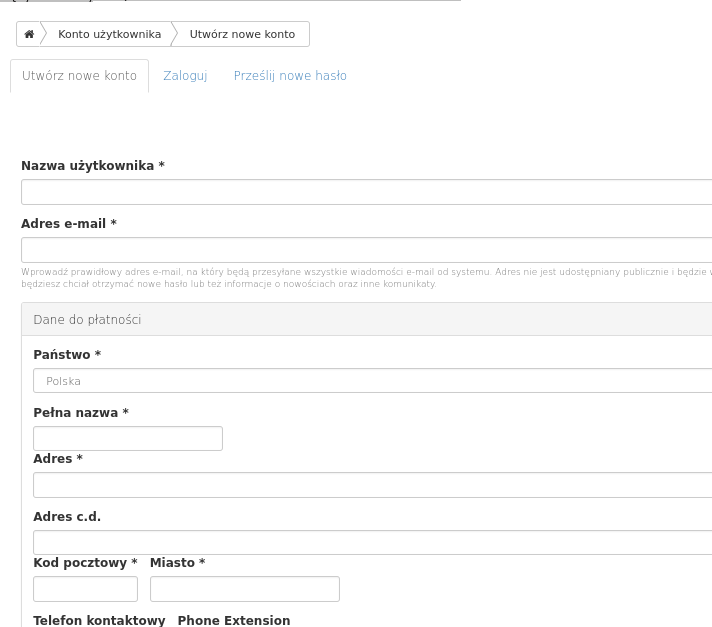
\includegraphics[scale=0.60]{register}
		\caption{Fragment strony rejestracji nowego użytkownika}
	\end{figure}
					
	\par Menu sklepu ułożone według najczęściej wyszukiwanych kategorii zapewnia łatwość nawigacji.
					
	\begin{figure}[H]
		\centering
		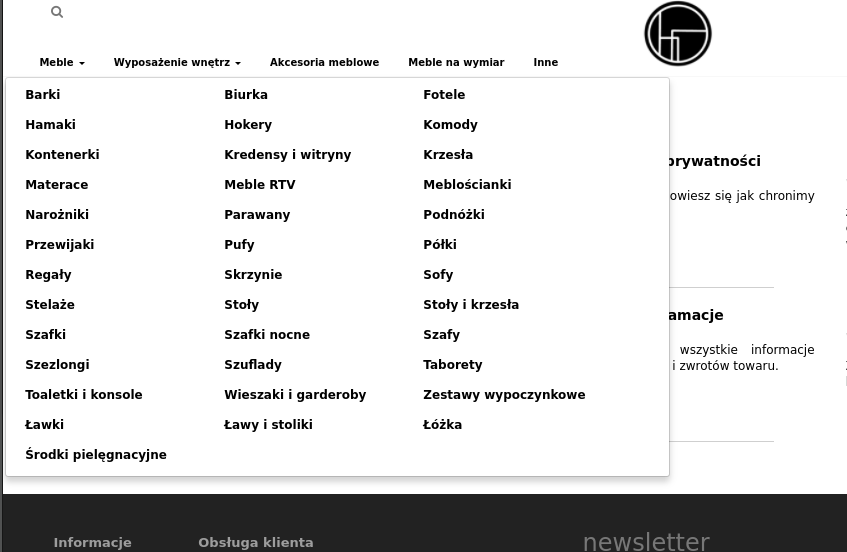
\includegraphics[scale=0.60]{menu}
		\caption{Menu sklepu}
	\end{figure}
 
